\documentclass{amsproc}


%%----------------------------
%%%% packages
%%----------------------------



\usepackage[utf8]{inputenc}   % For UTF-8 encoding
\usepackage{amssymb}            % AMS Symbols
\usepackage{amsmath,amsthm}     % AMS for Maths equations
\usepackage{bm}                 % bold math
\usepackage{braket}             % Bra-Ket Notation
\usepackage{subcaption}
\usepackage[a4paper,margin=26mm]{geometry}
\usepackage{graphicx}           %Graphics & Images
\usepackage{tikz}
\usepackage{listings}
\usepackage{hyperref}           %Hyperlinks


%%----------------------------
%%%% new-commands
%%----------------------------


\newcommand{\ITensor}{\texttt{ITensor}}
\newcommand{\julia}{\texttt{Julia}}

%%----------------------------
%%%% bibliography management
%%----------------------------

\lstset{
  basicstyle=\ttfamily,
  columns=fullflexible,
  breaklines=true}

\usepackage[
  backend=biber,
  style=phys,
  doi=true,
  eprint=true,
  url=false,
]{biblatex}



% Header files to maintain bibresources
% Be careful about the path



\addbibresource{./.src/.bib/adam-mipt.bib}
\addbibresource{./.src/.bib/arnau-fisher-info.bib}
\addbibresource{./.src/.bib/artiaco-info-lattice.bib}

      


%%---------------------------
%%%% Titles:
%%---------------------------


\title{Discrete Time Crystal: The Vanilla Unitary as a Brickwall Circuit}                        % model-dtc

%\title{Project Details: Charcterization of the Time-Crystal Criticality}                        % proposal-dtc
%\title{Physics of good Q-LDPC Codes}


\author{Sagnik Ghosh}
\address{Physikalisches Institut der Universit{\"a}t Bonn, Nu{\ss}allee 12, 53115 Bonn, Germany}


\date{December 27, 2023}            % model-dtc


%%---------------------------
%%%% Main Doc:
%%---------------------------

\begin{document}


\newtheorem{defn}[]{Definition}
\newtheorem{obs}[]{Observation}
\newtheorem{lem}[]{Lemma}
\newtheorem{thm}[]{Theorem}
\newtheorem{corr}[]{Corollary}
\newtheorem{conj}[]{Conjecture}
\newtheorem{prop}[]{Property}
\newtheorem{appr}[]{Approximation}
\newtheorem{claim}[]{Claim}
\newtheorem{notes}[]{Note}




\includegraphics[scale=0.03]{./.src/header/UNI_Bonn_Logo_Standard_RZ_Office.jpg}
%
\includegraphics[scale=0.95]{internal-lhead.png}
%\includegraphics[scale=0.83]{internal-lhead-detailed.jpeg}

\vspace{6mm}

\maketitle

%%----------------------------
%% DTC-Model
%%----------------------------

\section{Model}

The model we will be concerned with is the brick-wall circuit from Ipolitti et al \cite{Khemani2021DTCinNISQ,ippolitti2022time}. The General Floquet Model considered here, that exhibits a Discrete Time Crystal in 1D is an disordered Ising model with periodic $\pi/2$ Kicks about the $x$-axis. The system is probed only at stroboscopic times, $t=n \tau$, and $\tau=1$

\begin{equation}
    U_F= e^{-ig\sum_i X_i}e^{-i\tau(\sum_{i} J_{i} Z_i Z_{i+1}+H_{int})}e^{-i\tau(\sum_{i} h_{i} Z_i)}
\end{equation}

Here we have adopted the standard information theoretic notation (i.e have denoted Pauli operator $\sigma^Z_i=Z_i$ etc.) The $H_{int}$ denotes some generic interaction such as fields or coupling, 

\begin{equation*}
\begin{split}
    H_{int}&=  \frac{\theta}{2}\sum_{i}[X_iX_{i+1}+Y_iY_{i+1}] \text{(XY Coupling)}
\end{split}
\end{equation*}


\begin{figure}[h]
\begin{subfigure}{0.59\textwidth}
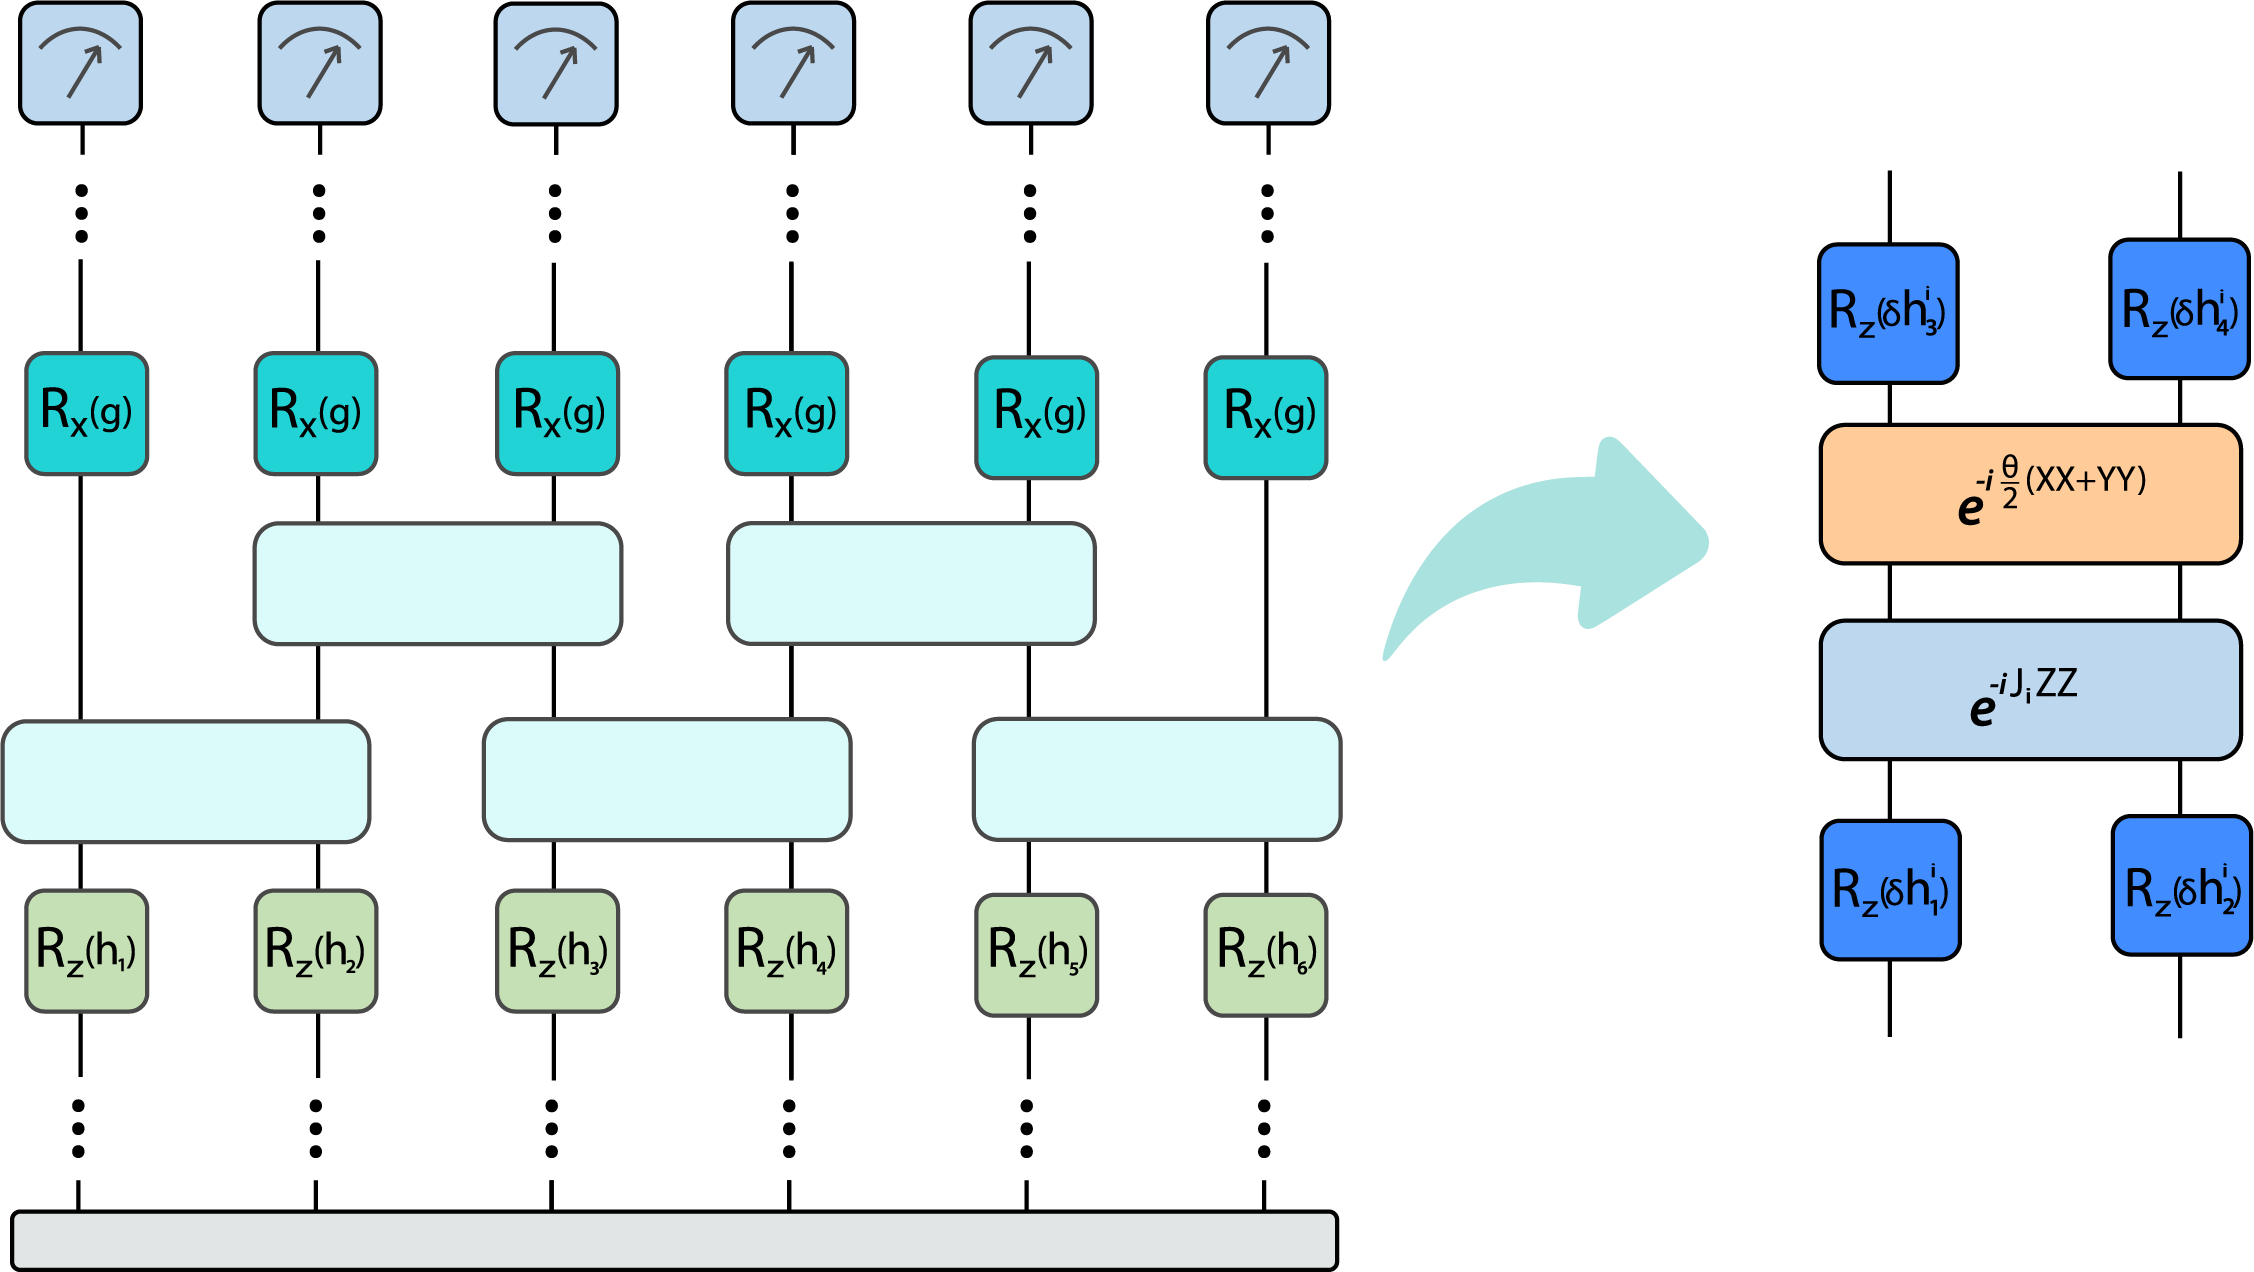
\includegraphics[width=0.9\linewidth]{./.src/images/DTC_circuit.png} 
\label{fig:subim2a}
\end{subfigure}
\begin{subfigure}{0.39\textwidth}
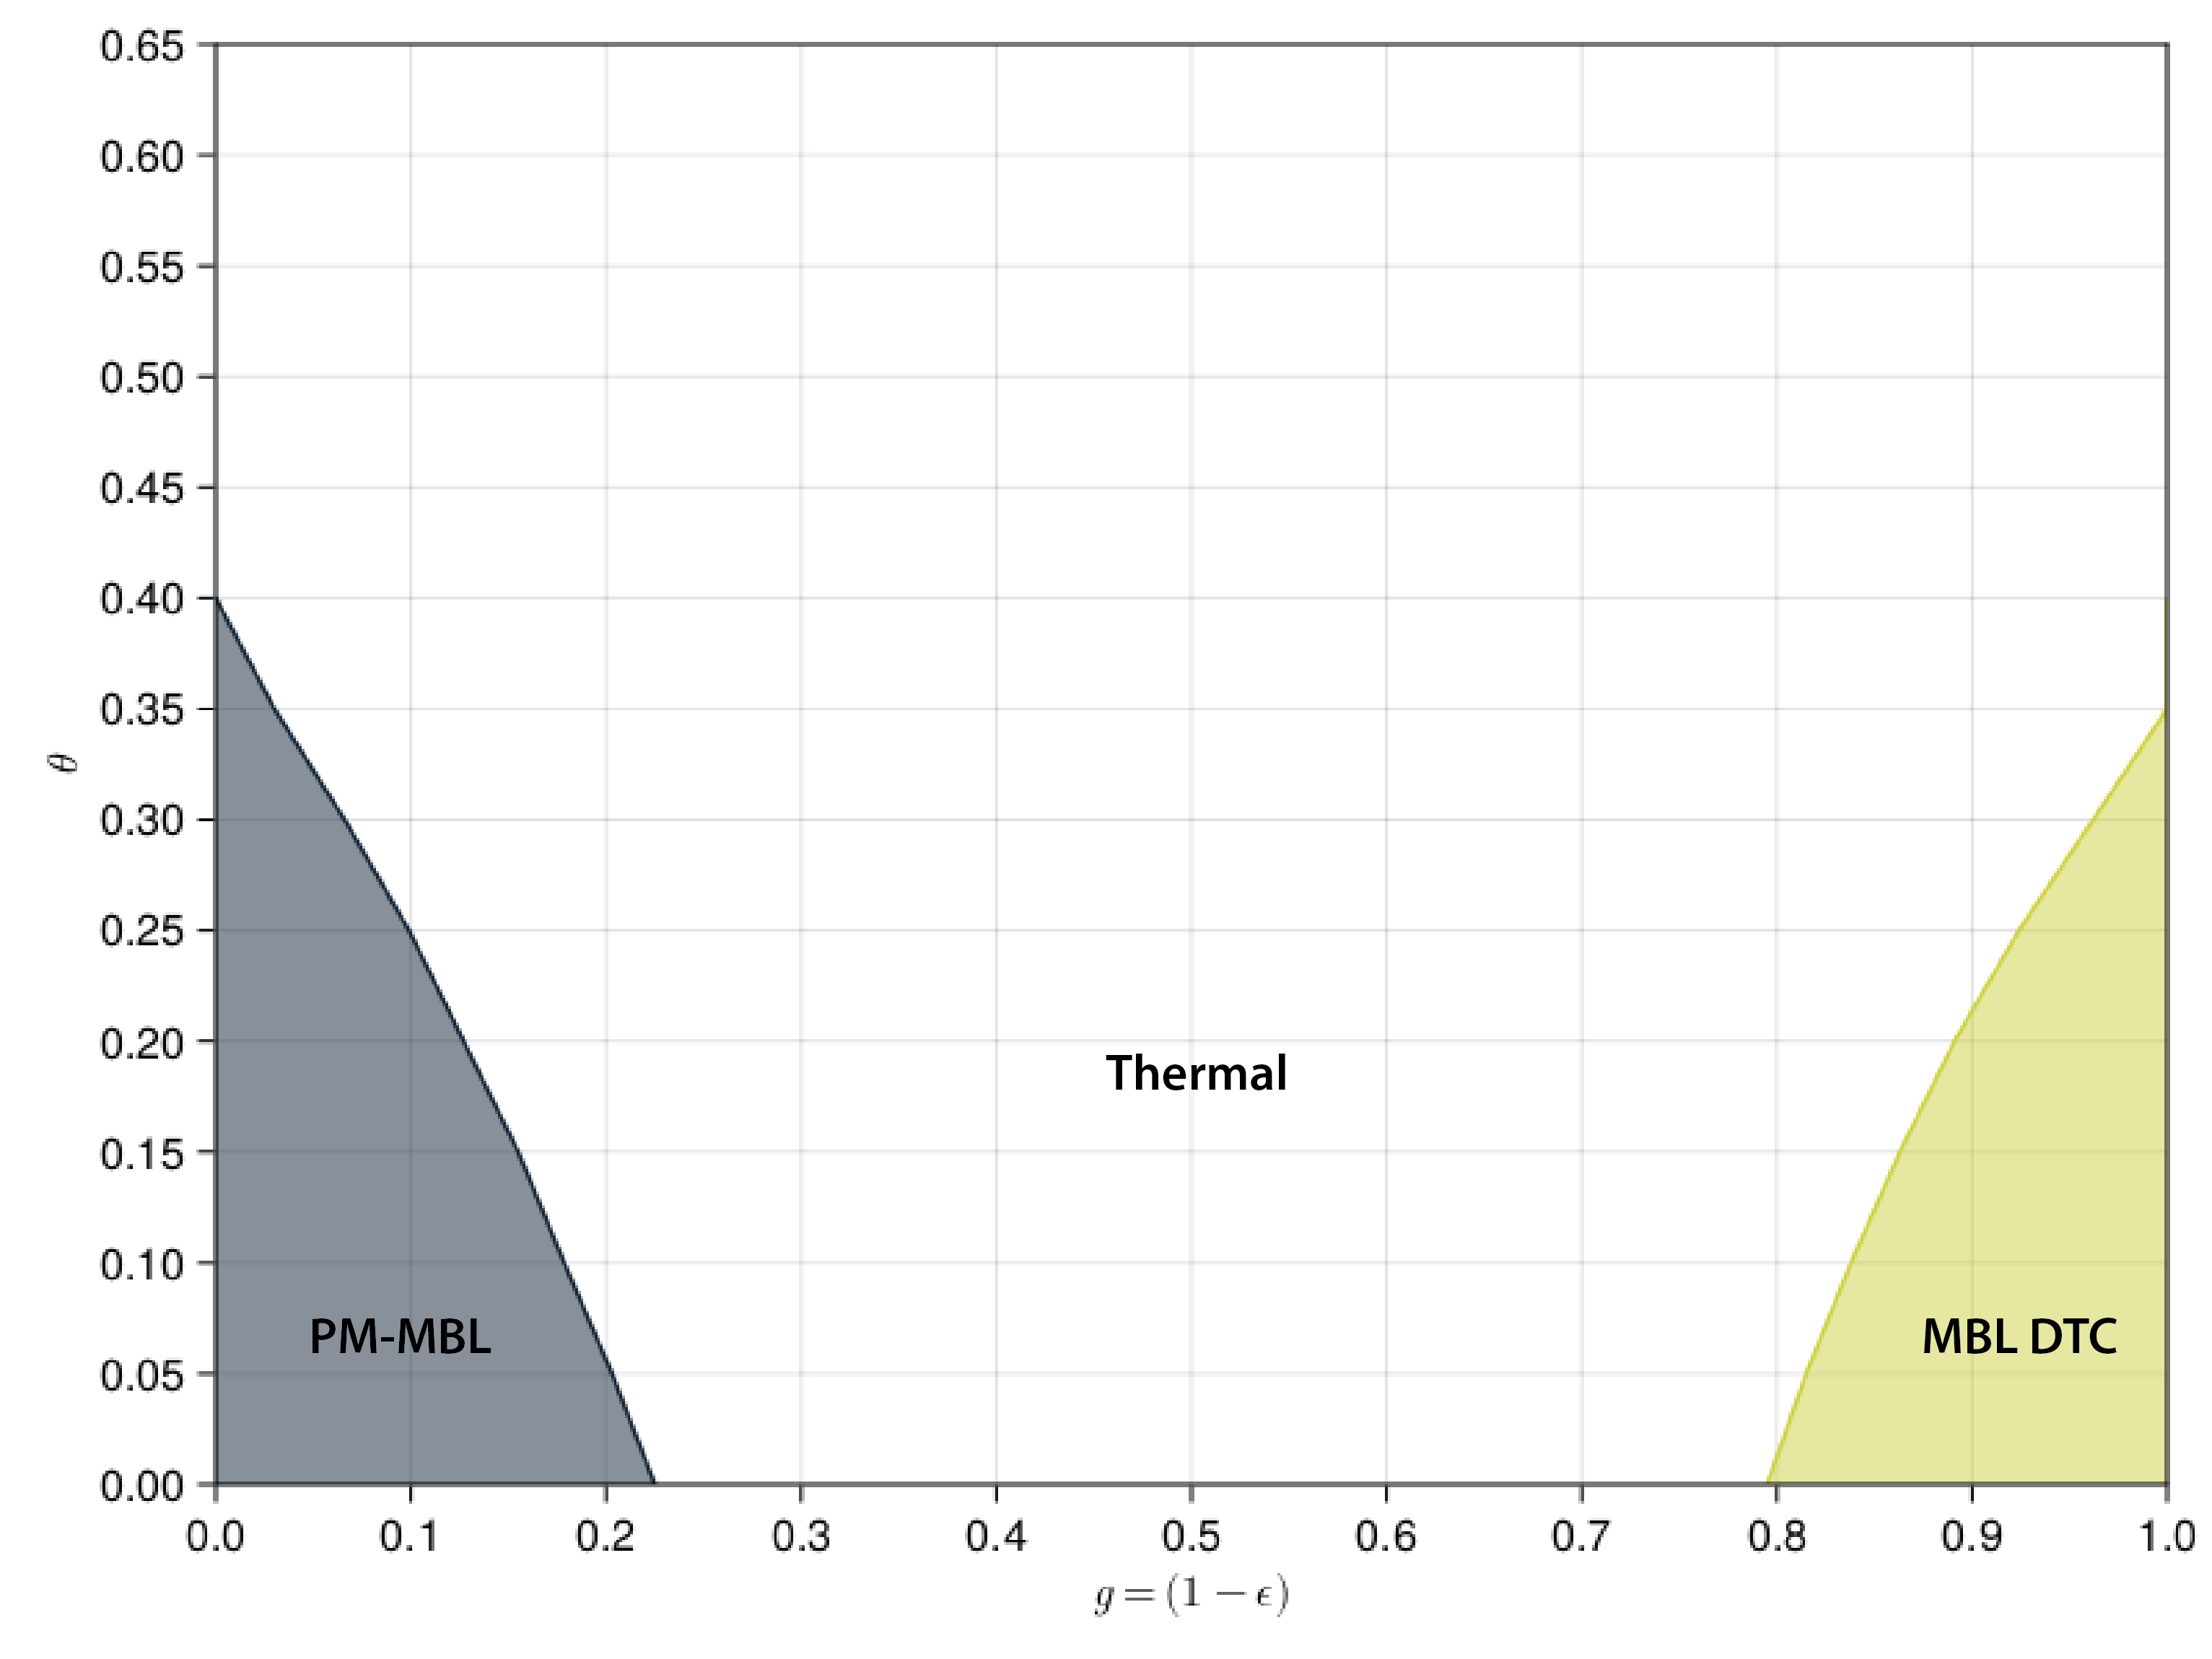
\includegraphics[width=0.9\linewidth]{./.src/images/Phase_diagram_Labeled.png} 
\label{fig:subim2a}
\end{subfigure}
\caption{Schematic representation of the circuit and the associated phase diagram. The circuit exhibit three phases. For smaller values of $\theta$ and $\epsilon$ close to 1, that is $g$ close to 0, it can support a MBL phase which is paramagnetic in nature. For small $\theta$ and $\epsilon$ close to 0, that is $g$ close to 1, it supports a DTC MBL phase with a period multiplicity of 2. In the middle region the system tend to scramble. The phase boundary was extracted from results of \cite{Khemani2021DTCinNISQ}, and was obtained from finite size scaling of the disorder averaged level spacing ratio.} 
\end{figure}

Among these parameters $J_i, h_i$ are disordered and are uniformly sampled from $[0,\frac{\pi}{2}]$ to ensure localisation and thereby to prevent the system from heating up to triviality from the kicks \cite{Khemani2015phasestructre}. In absence of interaction and with perfect kicks it is trivial to see that operators of the form $\braket{Z(0),Z(n)}$ breaks the discrete time symmetry and exhibits a period doubling. The non-triviality of the DTC as a \textit{phase} comes from the fact that this feature persists strongly even in the presence of interactions as well as with imperfect kicks (i.e $g=\frac{1}{2}=(\pi-\epsilon)$ with finite but small $\epsilon$). 

In a quantum device this is realised as a brick-wall circuit. 

%insert image of circuit

We also add further small uncertainties in the realisations of the two body gates 

\begin{equation}
    \theta=[\Bar{\theta}-\frac{\Delta\theta}{2},\Bar{\theta}+\frac{\Delta\theta}{2}]
\end{equation}

where $\Delta\theta=\frac{\pi}{50}$ and random single body $Z$ gates, $RZ(\Delta h)$, to both the legs before and after the application of the two body gates. $\Delta h=\frac{\pi}{50}$.
                   % model-dtc



%%----------------------------
%% DTC-Propoal
%%----------------------------



%\section{Introduction}

Here is a rough tl;dr about what this document is about. As can be read in \cite{Arnau2025MultipartiteEntanglementPhysRevLett} Arnau et. al. had developed a possible interesting way to use the fisher information as a tool to charecterise the scrambling-purifying transitions especially in the context of monitored quantum circuits. The very rough idea of how that works is as follows; 

It is well known that both product states and maximally entangled states has exponentially decaying correlations. The construction of Arnau et. al. specifically exploits this fact that, the for any such exponentially decaying correlated state, under finite-size scaling the fisher information of well chosen operators stays finite, the hope here is, normally around a critical state, we have scale invariance and hence algebrically correlated states, and hence the fisher information of well chosen operators should diverge under finite-size scaling. This is kind of smart in a sense, especially in context of monitored quantum circuits, where the transition is otherwise hard to charecterise. But the catch here is for this to work, one needs to ensure that we are probing correlations that are not exponentially decaying.


\begin{notes}[Questions:]    
1. Is this way of probing things post-selection free?\\
2. How to choose the operators?\\
3. Can we actually show that the maximal divergence of fisher information is achived exactly at the critical point, that is for a conformal state?
\end{notes}

Anyhow, with some further applications of this measure in context of monitored random circuits the method ran into a problem, and the resolution seemed to be that a Random unitary brickwall always generated maximally entangled states, and although local projections disentangles the qubits, on which the measurements were carried on, the rest of the system still remained maximally entangled, and hence the fisher information of any local operator always remained finite. This was kind of a bummer, and one possible way out seems like to use scramblers that generates algebrically correlated states perforated with local projections. The bet is that, in such a scenario, the fisher information of well chosen operators should diverge at the critical point, as it is specifically designed to do so.

On a systematic level, it is clear that the fisher information is designed to probe correlations of states, that falls exactly in the regime of \textit{entanglement barrier}. And it seemed like the most natural choice to decode the physics behind this was to use the \textit{information lattice} by Artiaco et. al. \cite{Artiaco2024EfficientLargePRXQuantum}, which is specifically designed to probe the information content and entanglement structure of a quantum many-body state at various length scales. 


Information lattice is one of the most elegant way to prove scale invariance and algebric correlations of many-body states. The idea behing the document is to use the information lattice to find physical scramblers that generates algebrically correlated states. And then the bet is, the Fisher information of Arnau would be super efficient in picking up the criticality of the scrambling-purifying transition in these monitored quantum circuits.


\begin{notes}[Food for further thoughts:]
Before moving on to the details, here is a few pointers, that I personally think are really interesting food for thought for the whole game of measurement induced phase transitions in general. Although, obviously the finite size scaling of entanglement entropy growth seems to show a criticality, very clearly this is not at the level of states, as absolutely no states are conformal at any point in the phase diagram. That raises a few questions, for example, is this actually even second order, and if it is, then what is the relevant unconstrained phase-space. This concerns are of course not new, as we know that this is also exactly why this kind of criticalities suffer from post-selection problems. It is also extremely related to the questions why constructing the replica theory for these systems needs a different normalisation (the Born Rule factor) and also why the resultant Landau-Ginzburg theories \cite{Adam2021MeasurementEntanglementPRXQuantumTheTheoryOfEverythingPaper} actually do not have the correct symmetries of the original problem \footnote{ Adam Nahum, private communication, (\textit{Damn! I have been waiting to write this line!})}.
\end{notes}             % proposal-dtc 
%\input{proposal/processing}        % proposal-dtc 
%\input{proposal/connecting}        % proposal-dtc 
%\input{proposal/enabling}          % proposal-dtc 



%%----------------------------
%% QLDPC
%%----------------------------

%\input{Q-LDPC/defn}


%%----------------------------
%% End:
%%----------------------------

\printbibliography

\end{document}
